% JuliaCon proceedings template
\documentclass{juliacon}
\setcounter{page}{1}
\usepackage{amsmath}
\usepackage{cleveref}
\usepackage{microtype}
% \usepackage{fontspec}

%% extra links:
%% - GPU Julia: https://cuda.juliagpu.org/stable/tutorials/introduction/
%% - GPU x2: https://nextjournal.com/sdanisch/julia-gpu-programming
%% - NaN vs missing https://discourse.julialang.org/t/is-there-any-reason-to-use-nan-instead-of-missing/84396

% If using Emacs, put cursor on last closing paren and call "eval-last-sexp" (usually `C-x C-e') to regenerate
% (save-excursion
%  (let* ((toc (funcall imenu-create-index-function))
%         (headers (mapcar (pcase-lambda (`(,str . ,loc)) str)
%                          toc)))
%    (beginning-of-buffer)
%    (search-forward (concat "%% " "--- autogenerated TOC ---"))
%    (next-line)
%    (beginning-of-line)
%    (let ((start (point)))
%      (search-forward (concat "%% " "--- end autogenerated TOC ---"))
%      (beginning-of-line)
%      (delete-region start (point))
%      (goto-char start))
%    (cl-loop for header in headers
%             do (insert (format "%% %s\n" header)))
%    (next-line)))

%% --- autogenerated TOC ---
% juliacon
% document
%   Introduction
%   Floating Point Exception Primer
%     Where do \NaN{
%       TODO good quote, try to work this in
%     Infinity
%     To Kill a Floating Point
%   \FlowFPX{
%     \FT{
%       Tracking Excptional Values
%       Fuzzing
%     Visualization
%     \GPUFPX{
%   Case Studies
%     Surprise \NaN{
%       CSTGs help us get a bigger picture
%     \NaN{
%     Finch
%     A Bug-Hunting Safari
%     \GPUFPX{
%   Related Work
%   Discussion
%     Tracking more than \NaN{
%     Enhanced Fuzzing
%     Static FPX, Gradual Types
%   Acknowledgments
% document
%% --- end autogenerated TOC ---

\begin{document}

% Misc typographical tweaks.
\setlength{\parindent}{1.2em}
% \setmonofont{JuliaMono}[Extension = .ttf, Path = ./, UprightFont = *-Regular, ItalicFont = *-Italic]

% **************GENERATED FILE, DO NOT EDIT**************

\title{My JuliaCon proceeding}

\author[1]{Taylor Allred}
\author[1]{Xinyi Li}
\author[1]{Ashton Wiersdorf}
\author[1]{Ben Greenman}
\author[1]{Ganesh Gopalakrishnan}
\affil[1]{University of Utah}

\keywords{Julia, Optimization, Game theory, Compiler}

\hypersetup{
pdftitle = {My JuliaCon proceeding},
pdfsubject = {JuliaCon 2019 Proceedings},
pdfauthor = {1st author, 2nd author, 3rd author},
pdfkeywords = {Julia, Optimization, Game theory, Compiler},
}


\maketitle

\begin{abstract}
  Reliable numerical computations are central to high-performance computing and machine learning.
  We present FlowFPX: a tool set for debugging floating-point code.
  FlowFPX is composed of two primary parts: FloatTracker, a Julia-based tool for tracking the onset and flow of floating-point exceptions; and CSTG, a stack trace visualizer.
  FlowTracker's design exploits Julia's operator overloading to trace exception flows and even inject exceptions to accelerate testing.
  We present intuitive visualizations of summarized exception flows including how they are generated, propagated and killed, thus helping with debugging and repair.
\end{abstract}

\newcommand{\code}[1]{\texttt{#1}}
\newcommand{\FlowFPX}{FlowFPX}
\newcommand{\GPUFPX}{GPU-FPX}
\newcommand{\FloatTracker}{FloatTracker}
\newcommand{\FT}{\FloatTracker}
\newcommand{\Fp}{Floating-point} % hyphen or no?
\newcommand{\fp}{floating-point} % hyphen or no?
\newcommand{\CSTG}{stack graph}
\newcommand{\CPP}{\code{C++}}
\newcommand{\Dendro}{\textsc{Dendro}}
\newcommand{\urlaccess}[2]{\url{#1}}
\newcommand{\Nan}{\code{NaN}}
\newcommand{\NaN}{\Nan}
\newcommand{\Inf}{\code{Inf}}
\newcommand{\zerowidth}[1]{\makebox[0pt][l]{#1}}
\newcommand{\zerocode}[1]{\zerowidth{\code{#1}}}

\section{Introduction}

Reliable numeric computations are central to high-performance computing,
machine learning, and scientific applications.
Yet, the \fp{} arithmetic that powers these computations is fundamentally
unreliable~(\cref{s:background}).
Exceptional values, namely Not a Number (\Nan{}) and infinity (\Inf{}),
can and often do arise thanks to culprits such as roundoff error,
catastrophic cancellation, singular matrices, and vanishing
derivatives~\cite{sdjmrstp-pc-2022,ddghlllprr-correctness-2022,gllprt-correctness-2021,fpchecker-reports,llg-soap-2022,bllmg-xloop-2022}.
When exceptions happen, domain experts must take time away from their main
focus and trek down a rabbit hole to find the source of the error.
There is little tool support to assist in this difficult task,
thus (unsurpringly) a quick GitHub search reports over 4,000 open issues
related to \NaN{} or \Inf{} exceptions~\cite{github-issues}.

We introduce \FlowFPX{}, a toolkit for debugging
\fp{} exceptions in an easy and intuitive way~(\cref{s:flowfpx}):
\begin{itemize}
  \item
    The centerpiece of \FlowFPX{} is \FT{}, a dynamic analysis tool that uses
    Julia's operator overloading to selectively monitor for exceptions and to
    fuzz code for vulnerabilities.
  \item
    To visualize results, \FT{} adapts coalesced stack-trace graphs 
    (CSTGs, or \CSTG{}s)~\cite{hmbdrg-cse-2014} for a whole-program view on the generation,
    propagation, and death of exceptional values.
  \item A companion tool \GPUFPX{}~\cite{llsflg-hpdc-2023} provides fine-grained insights for GPU kernels.
\end{itemize}
%
Together, the \FlowFPX{} tools have helped debug exceptions in a variety
of applications: from ocean simulations to heat models~(\cref{s:casestudies}).
That said, there is much more to explore.
\FlowFPX{} is a growing project and we welcome feedback from domain experts
on how to best suit their workflow.

This paper concludes with related work~(\cref{s:related}) and a
brief discussion~(\cref{s:discussion}).


\section{Floating Point Exception Primer}
\label{s:background}

%% TODO use the GPU-FPX paper as a guide for the background. Give a little more detail than that, but not much!

% TODO: talk about how floating point != real numbers → errors appear and build up
% (see other tutorials; Art of Computer Programming, Ganesh, slides in Google Drive from guy in England)
% 2 paragraphs or so: floating point primer

\Fp{} numbers are a way of representing real numbers in a computer.
However, since we limit our precision to a fixed, finite set of bits, \fp{} values are \emph{inherently approximate} and necessarily incur some error during computation.
This is not bad; it is a trade-off: we get fast and compact representations that are good enough for most use cases.
However, the downside is that \fp{} numbers \emph{do not} behave like real numbers.

% FIXME: more resources!
There are many excellent resources\cite{knuthArtComputerProgramming1997,torontoPracticallyAccurateFloatingPoint2014} on understanding the theory behind \fp{};
we will explain the most essential aspects here briefly.

A \fp value approximates real number $r \in \mathbb{R}$ by expressing $r$ in scientific notation $r = s \times f \times b^{e-q}$,
for some base $b$,
an integer exponent $e \in \mathbb{N}$,
a fixed value called an \emph{excess} $q$,\footnote{The purpose of the excess $q$ is so that with value of $e > q$ we can represent positive exponents, and $e < q$ we can represent negative exponents.}
a \emph{sign} $s \in \{-1, 1\}$,
and a \emph{fraction} $f$ such that $0 \leq f < b$.\footnote{Another name for the fraction part commonly seen in the literature is ``mantissa'' or ``significand''.
  You might occasionally also see ``characteristic'' referring to the exponent.
  We will stick to ``fraction'' and ``exponent'' however.}

We pack $s$, $e$, and $f$ into bit fields.
This gives us a compact representation for both very small and very large values: because the exponent is variable, we can represent numbers as big as Avogadro's number or as small as Planck's constant with the same number of bits.
However, since we have only a finite number of bits $p$, we have to round $f$ and the range of $e$ is limited.
Moreover, there is some error between the real number $r$ and the value we can express with a float.
This is why $0.1 + 0.2 = 0.30000000000000004$---$0.3$ is not precisely representable.

To make matters worse, things get tricky when we do math.
Adding e.g. Avogadro's number and Planck's constant together is beyond 16-, 32-, and 64-bit floats to represent.
In fact, whenever the exponents differ by more than $p+2$, the result of the addition will just be the same as the larger number.
In the case of Avogadro's number, adding any value less than $FIXME$ will just result in Avogadro's number again.

The gradual accumulation of these errors and other representation issues leads to surprising results!
% FIXME: more examples of a NaN popping up out of nowhere, e.g. with bad addition

In our work we focused on two of the most common problematic values in the \fp{} space: \NaN{} and \Inf{}.
We leave the possibility of tracking other kinds of troublesome values (e.g. subnormal numbers) open, but for our work we restrict ourselves to just these values.

\subsection{Where do \NaN{}s come from?}

IEEE 754~\cite{IEEEStandardBinary1985} lists the following operations (among a few others) where \NaN{}s result:

\begin{figure}[h]
  \label{fig:nan-gens}
  \begin{itemize}
  \item $\frac{0}{0}$ or $\frac{\infty}{\infty}$
  \item $0 * \infty$
  \item $x \% y$ when $x = \infty$ or $y = 0$
  \item $+\infty + -\infty$ or $\infty - \infty$
  \item The square root or logarithm of a negative number
  \end{itemize}
  \caption{\NaN{}-producing operations}
\end{figure}

When one of these events happens, we call it a \NaN{} \emph{generation}.

Most mathematical operations preserve \NaN{}s.
We call these instances \NaN{} \emph{propagation}, as the \NaN{} is propagated from the source in the arguments to the result.

There are, however, some instances where the IEEE standard requires that \NaN{}s to \emph{not} propagate from arguments to the result; we call these \NaN{} \emph{kills}.
Sometimes this can be good---an \texttt{isnan} check should clearly return a boolean and not a \NaN{}---but kills are often harmful in two ways:

\begin{enumerate}
  \item Users no longer see that there was some errant operation: \NaN{}s are an opportunity to closely examine data for problems and code for unsoundness.
  \item \NaN{} kills can influence the control of a program leading to incorrect results, as we saw in~\cref{s:to-kill-a-fp}.
\end{enumerate}

Here are cases where, according to the IEEE standard, a \NaN{} can be killed:

\begin{align*}
x \; \texttt{cmp} \; y &\rightarrow false &\text{where \texttt{cmp} is \texttt{<}, \texttt{>}, \texttt{<=}, etc.} \\
1^{\text{\texttt{\NaN{}}}} &\rightarrow 1 \\
\text{\texttt{\NaN{}}}^{0} &\rightarrow 1
\end{align*}

FloatTracker monitors these and all other operations for interesting events.

\subsubsection{TODO good quote, try to work this in}

From IEEE 754. Section 6.2 here: \url{http://www.dsc.ufcg.edu.br/~cnum/modulos/Modulo2/IEEE754\_2008.pdf}:

\begin{quote}
  Quiet NaNs should, by means left to the implementer’s discretion, afford
  retrospective diagnostic information inherited from invalid or unavailable
  data and results.
\end{quote}

Found via \url{https://anniecherkaev.com/the-secret-life-of-nan}

TODO what other tools are there for retrospective diagnosis?

\subsection{Infinity}

%%ben: shouldn't this come before NaN b/c infs lead to NaNs?

There are two infinities, $+\infty$ and $-\infty$, but they behave the same for our purposes, so we will refer to them just as ``\Inf{}''.
Like \NaN{}s, \Inf{} can crop up when bad math happens: $\frac{x}{0} \rightarrow \infty$ when $x \ne 0$.
\Inf{} can also arise when numbers get too big or too small for the choice of representation.

% Here is a short, illustrative example about the problem.
\subsection{To Kill a Floating Point}
\label{s:to-kill-a-fp}
% If anyone has a better "kill" pun/reference than "To Kill a Mockingbird", I'm all ears.

\begin{figure}
  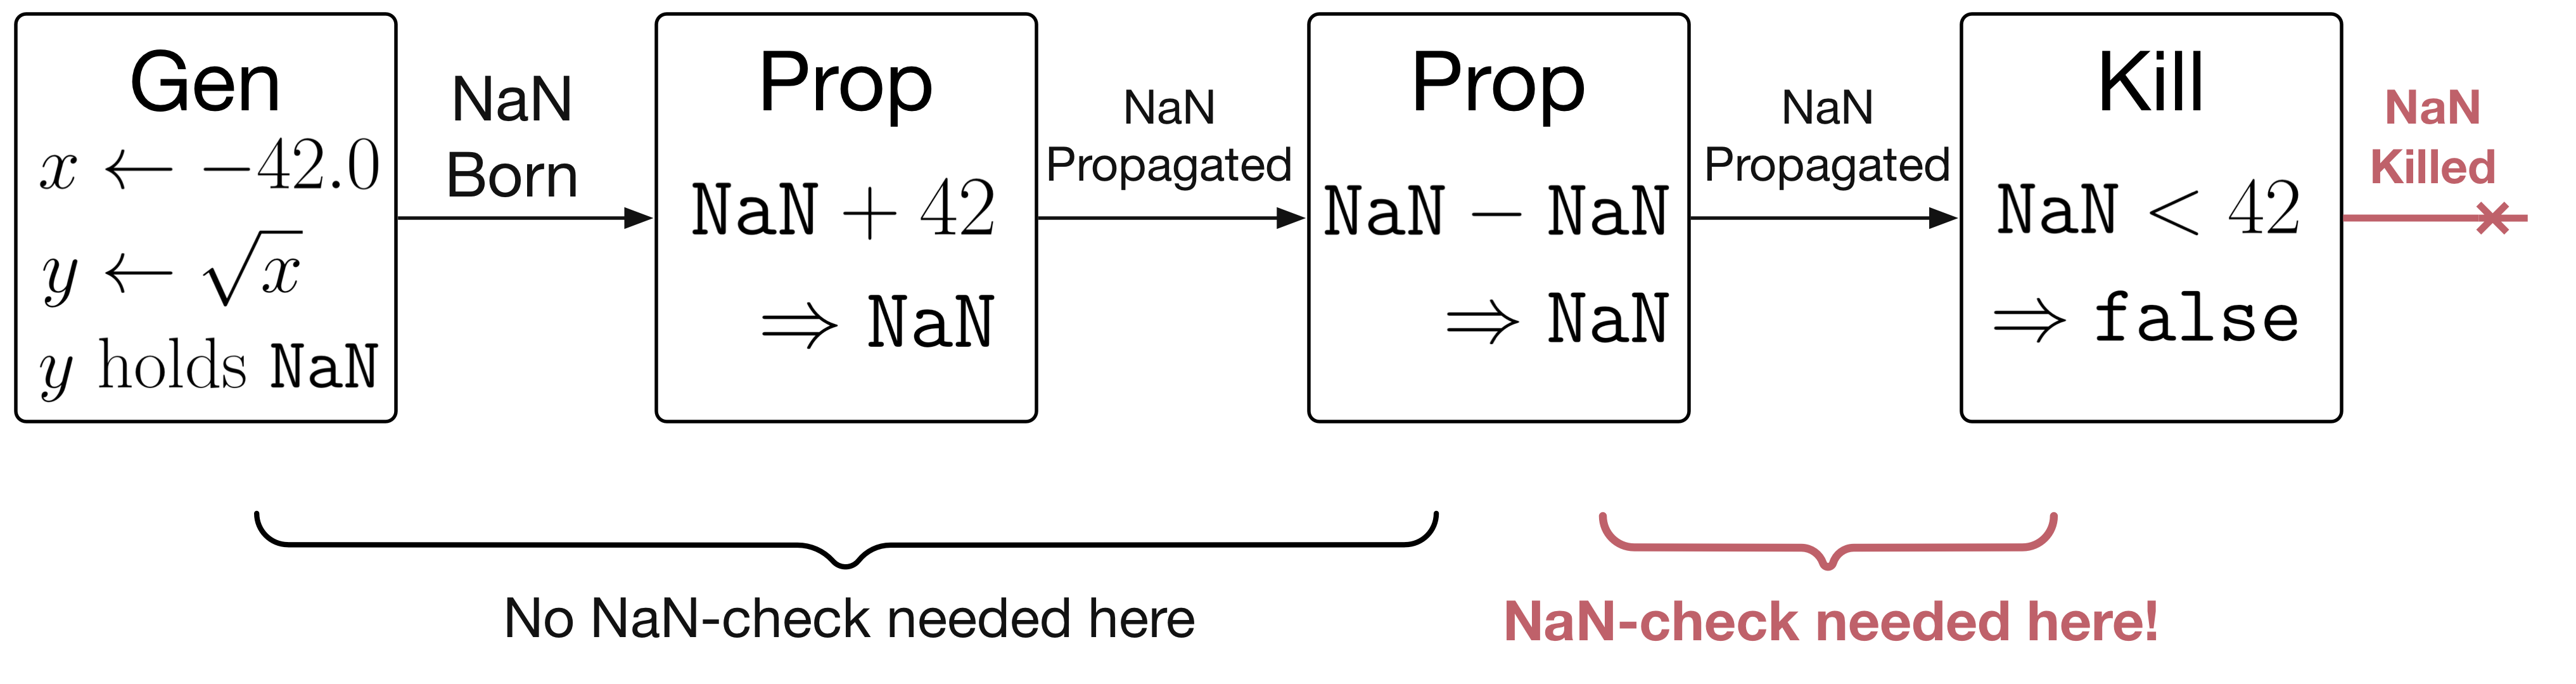
\includegraphics[width=\columnwidth]{fig/genpropkill-outline.png}
  \caption{Gen, Prop, Kill: Lifetime of a \NaN{} value}
  \label{f:gpk}
\end{figure}

The IEEE 754 specification for \fp{} numbers governs how \NaN{}s are handled as arguments to arithmetic functions~\cite{IEEEStandardBinary1985}.
Most of the time, when any or all of the arguments are \NaN{}, the result is also a \NaN{}.
This is good and desirable, because it means that an arithmetic error---even if buried deep in an expression---will still be observable, allowing a user to find and debug it.

However, there are a few places where \NaN{}s flow into an expression, but not out.
We call these instances ``\NaN{}-kills'', and these can lead to subtle logic bugs.
Consider the following example:

\begin{lstlisting}[language = Julia]
function bad_max(lst)
  max_seen = 0.0
  for x in lst
    if ! (x <= max_seen)
      # swap if new val greater
      max_seen = x
    end
  end
  max_seen
end

function good_max(lst)
  foldl(max, lst)
end
\end{lstlisting}

Both \texttt{bad\_max} and \texttt{good\_max} compute the maximum in a list.
However, the \texttt{<=} operator used in the \texttt{bad\_max} implementation does \emph{not} propagate \NaN{}s, so you might not get the result you expected:

\begin{lstlisting}[language = Julia]
bad_max([1, 5, NaN, 4])     # returns 4
good_max([1, 5, NaN, 4])    # returns NaN
\end{lstlisting}

Not only is the result from \texttt{bad\_max} problematic for obscuring the fact that there was a \NaN{} in the list, the result is also wrong!
The built-in \texttt{max} function correctly propagates \NaN{}s, so we can see from its return that we got a \NaN{} somewhere.
It's not entirely obvious \emph{where} that \NaN{} came from---but more on that later.   % this promise answered in "NaN propagation monitoring"

\section{\FlowFPX{}}
\label{s:flowfpx}

\FlowFPX{} is a growing set of tools to aid in tracking down \fp{} exceptions.
The two primary tools we cover in this paper are \FT{} and CSTG:

\begin{itemize}
\item \FT{}'s role is twofold: to trace the lifetime of exceptional \fp{} values and to enable inside-out fuzzing.
\item CSTG's role is to visualize the tracing output from \FT{} in compact form.
\end{itemize}

\GPUFPX\cite{llsflg-hpdc-2023} is another component of \FlowFPX{} that can track \fp{} exceptions inside a GPU kernel.
Please see the cited paper for more details on \GPUFPX.
Work to use \GPUFPX in tandem with \FT{} is ongoing.

%% TODO julia proposed consistent NaN handling,
%%  do we propagate the exact NaN
%%  https://github.com/JuliaLang/julia/issues/48523
%%
%% Ashton: @Ben we simply propagate whatever we got from the operation. If
%% Julia's behavior around an operator change, that should be preserved even
%% when using FloatTracker

\subsection{\FT{}}
\label{s:floattracker}

\FT{} has two roles:

\begin{enumerate}
  \item Track exceptional values
  \item Fuzz \fp{} code from the inside-out
\end{enumerate}

Building the mechanism to track exceptional values also gave us a way to inject exceptional values wherever \fp{} operations occur.
We will examine each of these roles, how they are used, and how \FT{} realizes them.

%% What it does, then how it works

\subsubsection{Tracking Exceptional Values}
\label{s:trackingexceptionalvalues}

\FT{}'s first purpose is to monitor \fp{} operations for exceptional values.
\FT{} interposes on every arithmetic operation and standard library call that involves a \fp{} and logs a stack trace to that point whenever an exception is generated, propagated, or killed.
A programmer can then use these stack traces to pinpoint where an exceptional value like \NaN{} came into being or where a guard against a \NaN{} kill is needed.
\FT{} can also log the arguments to the suspect call, so you can get \emph{normal, concrete} values to help you further discover what is going wrong.

All the logs that \FT{} captures are straight from Julia's \texttt{stacktrace()} function.
\FT{} writes these logs to file; one file for each kind of event.
This way, if a user of \FT{} is attempting to determine where a \NaN{} or an \Inf{} came from, they can look in the file for all the gen events.
Likewise, if the user wants to find where \NaN{}s get killed, then they can look in the kills file.

% note: there's a section on performance in the "discussion" section at the end, so we can leave it out here I think

While other tools like profilers might accomplish this tracking by writing extensions to the language's compiler or runtime, we were able to implement \FT{} entirely in user land.
We created custom types \texttt{TrackedFloat16}, \texttt{TrackedFloat32}, and \texttt{TrackedFloat64} that wrap their corresponding \texttt{Float16}, \texttt{Float32}, and \texttt{Float64} counterparts.
We then defined methods for every function in the \texttt{Base} module, including new implementations for operators like \texttt{+} and \texttt{*}.
This lets us intercept all \fp{} operations working on our \texttt{TrackedFloat} types.

\begin{lstlisting}[language = Julia]
function +(x::TrackedFloat64, y::TrackedFloat64)
  result = x.val + y.val
  check_error(+, result, x.val, y.val)
  TrackedFloat64(result)
end
\end{lstlisting}

These new methods had to be defined for every combination of tracked/untracked arguments;
fortunately Julia's metaprogramming abilities made it simple for us to scale without the code becoming unwieldy.
We made a macro that first loops through all the \texttt{TrackedFloat} types that we wished to implement, and then looped through all of the operators that we wished to support.
This approached saved us over 10x the lines a non-macro approach would have required.\footnote{We implemented overrides for 645 function/type combinations. At roughly 5 lines per variant, this is 3225 lines of code. Our implementation at time of writing weighs in at 218 lines of code, which is \emph{including} whitespace and comments.}
This approach was inspired by \texttt{Sherlogs.jl}.\cite{kMilanklSherlogsJl2021}

With the overrides in place, we can examine the arguments to a \fp{} operation to determine if an interesting event occurred.
Here is how we classify events around a \NaN{}:

\begin{center}
  \begin{tabular}{ccc}
    Arguments & Result & Event Type \\
    \hline
    No \NaN{} & \NaN{} & Gen \\
    \NaN{} & \NaN{} & Prop \\
    \NaN{} & No \NaN{} & Kill \\
  \end{tabular}
\end{center}

The same classification rules apply to \Inf{} and would apply to any other value of interest.

\subsubsection{Fuzzing}

The second role of \FT{} is to fuzz code from the inside out.
While it is wholly possible to fuzz a program by giving it random inputs, this might not help you find \emph{all} the places where an exceptional value could crop up during a calculation.\cite{ddghlllprr-correctness-2022}

The exception tracking infrastructure that we have gives us a simple way to inject exceptional values wherever we want in our code.
We have a global configuration system that allows us to turn on fuzzing and configure where, when, and how many \NaN{}s\footnote{At time of writing, \FT{} only injects \NaN{}, but it is trivial to extend the set of values to inject.} to inject.

\FT{} exposes these configuration options:

\begin{description}
\item[\texttt{active::Bool}] Inject only if this is true.
\item[\texttt{n\_inject::Int64}] Inject at most this many \NaN{}s.
\item[\texttt{odds::Int64}] Inject if \texttt{rand(odds) == 1}.
\item[\texttt{functions::Array}] Inject if we are within the dynamic extent of any of these functions.
\item[\texttt{libraries::Array}] Inject if the top-most stack frame\footnote{After stripping off the stack frames that come from \FT{} itself.} comes from any of these libraries.
\item[\texttt{replay::String}] Name of a file to read an injection recording from.
\item[\texttt{record::String}] Name of a file to write injection events to for later replay.
\end{description}

Then, each time we intercept a \fp{} operation, we check to see if we should inject a \NaN{}. First we check if we're replaying a recording: if we are, just do as the recording says. Otherwise, we check to make sure we have \NaN{}s remaining to inject and we roll a die to see if we should inject. We also check the current stack trace against the lists of functions and libraries to inject in. If all looks good, we inject.

In our experience, requesting the stack trace from Julia is the most expensive part of this operation.
Therefore, we defer the stack checks as late as we can.
Once the fuzzer runs out of \NaN{}s, it effectively turns off, so the rest of the fuzzing session proceeds much more quickly.
That said, gathering stack traces still incurs a heavy overhead during logging when interesting events occur;
we recommend limiting the number and kinds of events logged for optimal performance.

\subsection{CSTG}
\label{s:cstg}

Coalesced Stack Trace Graphs, or CSTGs\cite{humphreySystematicDebuggingMethods2014} provide a way to visualize large amounts of stack traces in a compact form.
\FT{} produces


\subsection{\GPUFPX{}}
\label{s:gpufpx}

FILL basic idea, loose coupling, typical overhead, 

% * what about GPUs? companion project at Utah GPU-FPX
% * architecture diagram, CPU + GPU, show Ocean source code
% * replace CPU() with GPU() in code, get output like below & attached

%% Ganesh
% 3) These are conceptually usable together (Julia calling GPU kernels below).
% The usage is simple: Start the Julia application that calls a GPU kernel under
% LD_PRELOAD as with GPU-FPX launch. When this launch transfers control to a GPU
% kernel, the GPU-FPX instrumentation starts notifying the exceptions on the
% console of the CPU. When the GPU launch returns, the exceptions go in the
% return call path of the Julia execution. Ashton and Xinyi plz validate this
% scenario



\section{Case Studies}
\label{s:casestudies}

\FlowFPX{} is effective for debugging all sorts of \NaN{}-related issues.
We have used it to reveal silent \NaN{}s, uncover the root cause of \NaN{}s,
and fuzz for weak points in several case studies.


\subsection{Surprise \NaN{}s: ShallowWaters}

Most physics simulations of this sort include a parameter called the Courant-Friedrichs-Lewy (``CFL'') parameter, which roughly describes the size of the time step to take in running the simulation.
Normally this value sits between 0 and 1---smaller values mean the simulation runs slower but with higher accuracy, whereas higher values mean the simulation takes bigger time steps and consequently runs faster, but results might be inaccurate.
The primary reason for problems arising comes from information not having enough time to propagate through the simulation before the next time step is taken.

It is not uncommon to encounter cases where setting the CFL parameter too high results in \NaN{}s in the result.
Driving the CFL parameter low enough to excise the \NaN{}s can make the simulation too long and unwieldy to be comfortable to use.
Identifying where \NaN{}s begin to arise can help point the way to where some mathematical refinement can be used to make the simulation both fast and accurate enough for practical use.

For our first case study, we looked at the \texttt{ShallowWaters} library~\cite{klowerNumberFormatsError2020,klowerPositsAlternativeFloats2019,klowerLowprecisionClimateComputing2021}, which runs a simulates the flow of water over a seabed.
This is not a general shallow waters simulation library---it is designed primarily to showcase numerical methods involving 16-bit floats.
That said, it works for our purposes as a proving ground for FloatTracker.
We dialed the CFL parameter up to high values (as high as 10) and we started seeing \NaN{}s in the result.
Note that the program did not crash: instead, it began producing bad output.

\begin{figure}
  \centering
  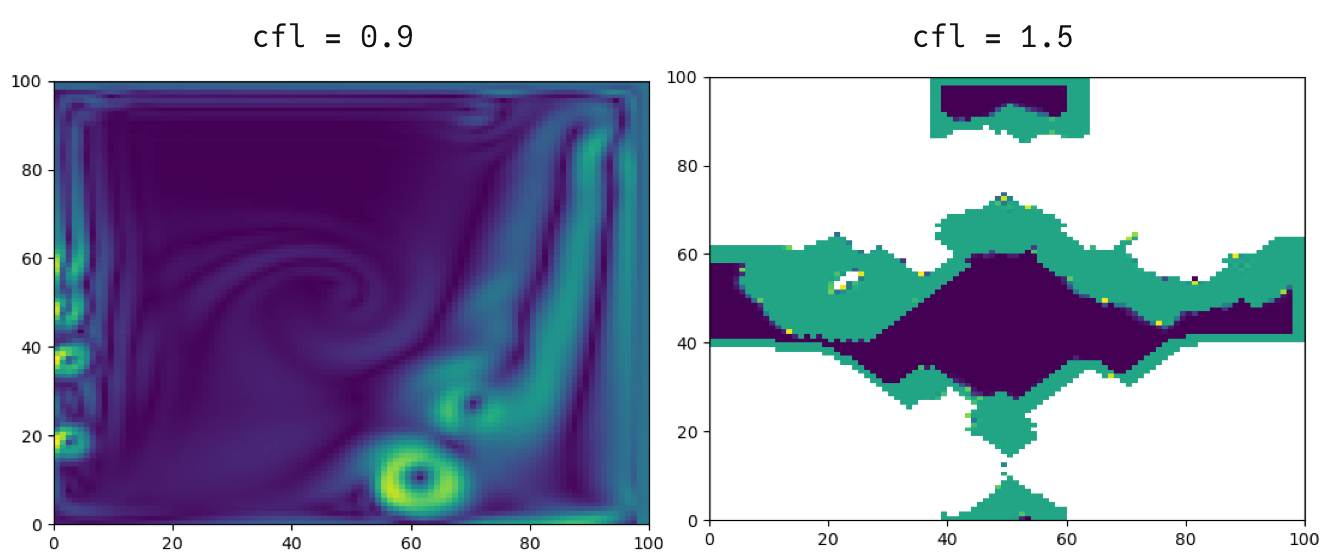
\includegraphics[width=3in]{./fig/shallow_waters_cfl_diff.png}
  \caption{Effect of high CFL parameters: on the left, normal output. On the right: \NaN{}s cause white holes and gaps in the result.}
  \label{fig:sw_nans}
\end{figure}

The holes in the plots are regions where \NaN{}s crept into the computation and destroyed the results.
In one regard, this is not as bad as a \NaN{} kill---knowing that there are \NaN{}s in the computation means that we have a chance to fix it, whereas a \NaN{} kill might silently give us the wrong answer.
Incidentally, we know that there were no \NaN{} kills in this test because our kill logs are empty.
But finding the sources of \NaN{}s can be tricky.
We expected \NaN{}s in this case because we set the CFL parameter up so high, but tracking down the sources of \NaN{}s generally is a difficult and time-consuming problem.

Fortunately in this case, one of the key features \texttt{ShallowWaters} is its \emph{type flexibility}:
\texttt{ShallowWaters} was designed to showcase physics simulations using variable levels of \fp{} precision.
Upon model construction, \texttt{ShallowWaters} allows you to specify a type for floats in the model.
We simply asked it to use our \texttt{TrackedFloat32} type, and then the entire simulation ran under the supervision of FloatTracker.

We ran ShallowWaters with a CFL value known to make bad outputs and recorded \NaN{} \texttt{gen} events:

\begin{lstlisting}[language = Julia]
set_logger(buffersize=20, cstg=true, cstgArgs=true,
           cstgLineNum=true)

P = run_model(T=TrackedFloat32,
              cfl=10, Ndays=100, nx=100, L_ratio=1,
              bc="nonperiodic",
              wind_forcing_x="double_gyre",
              topography="seamount")
\end{lstlisting}

This produced the following in the log file: (formatted for clarity)

\begin{verbatim}
…
-                 FT/TrackedFloat.jl:106
momentum_u!       ShallowWaters/rhs.jl:246
rhs_nonlinear!    ShallowWaters/rhs.jl:50
rhs!              ShallowWaters/rhs.jl:14 [inlined]
time_integration  ShallowWaters/time_integration.jl:77
run_model         ShallowWaters/run_model.jl:37
…
\end{verbatim}

We can see that the \NaN{} appeared from subtraction (first line) and that it was used in the \texttt{momentum\_u!} function on line 246 of the \texttt{rhs.jl} file (second line).
In figure~\ref{fig:nan-gens} we can tell that this must be the result of $\infty - \infty$.
Thus, with little effort we were able to track down where the \NaN{}s were originating.
Now the question is: where did the $\infty$ come from?

FloatTracker is not limited to \NaN{}s---we can track any kind of value that we want.
We have built-in support for tracking \NaN{} and $\infty$; we can look at the file of the $\infty$ gens where we see the following: (formatted for clarity)

\begin{verbatim}
check_error([-1.515f31, 2])  FT/TrackedFloat.jl:10
^(::TrackedFloat32, ::Int64) FT/TrackedFloat.jl:138
…
materialize(^)               broadcast.jl:860
top-level getproperty(P, :u) examples/sw_nan_tf.jl:14
…
\end{verbatim}

It looks like the $-\infty$ came from $-1.515e31^2$---no wonder a Float32 type couldn't handle something that large.
We can tell that because the first line shows us the arguments\footnote{There is a configuration option that allows us to control this behavior.} and the second line shows us what function got called. Moreover, we get the top-level line: we can see that it came from line 14 in our ShallowWaters file.

Tracking down why that value got so large is beyond the scope of FloatTracker right now.
Most likely we will need some domain-expertise to find a solution to this problem.
The point is, we were able to quickly and automatically arrive at this excellent starting point with FloatTracker.

\subsubsection{CSTGs help us get a bigger picture}

Running FloatTracker can produce a lot of logs.
To get a quick overview of the most common paths to problems, we can use CSTG to get an overview of what stack frames appear the most often.
% FIXME: cite CSTG

We can produce a CSTG of both the \Inf{} as well as the \NaN{} logs.
Here is what the two graphs look like:\footnote{As with the call stack logs, these have been edited for clarity. We only remove a few boxes in between—mostly due to space constraints in this paper.}

\begin{figure}
  \centering
  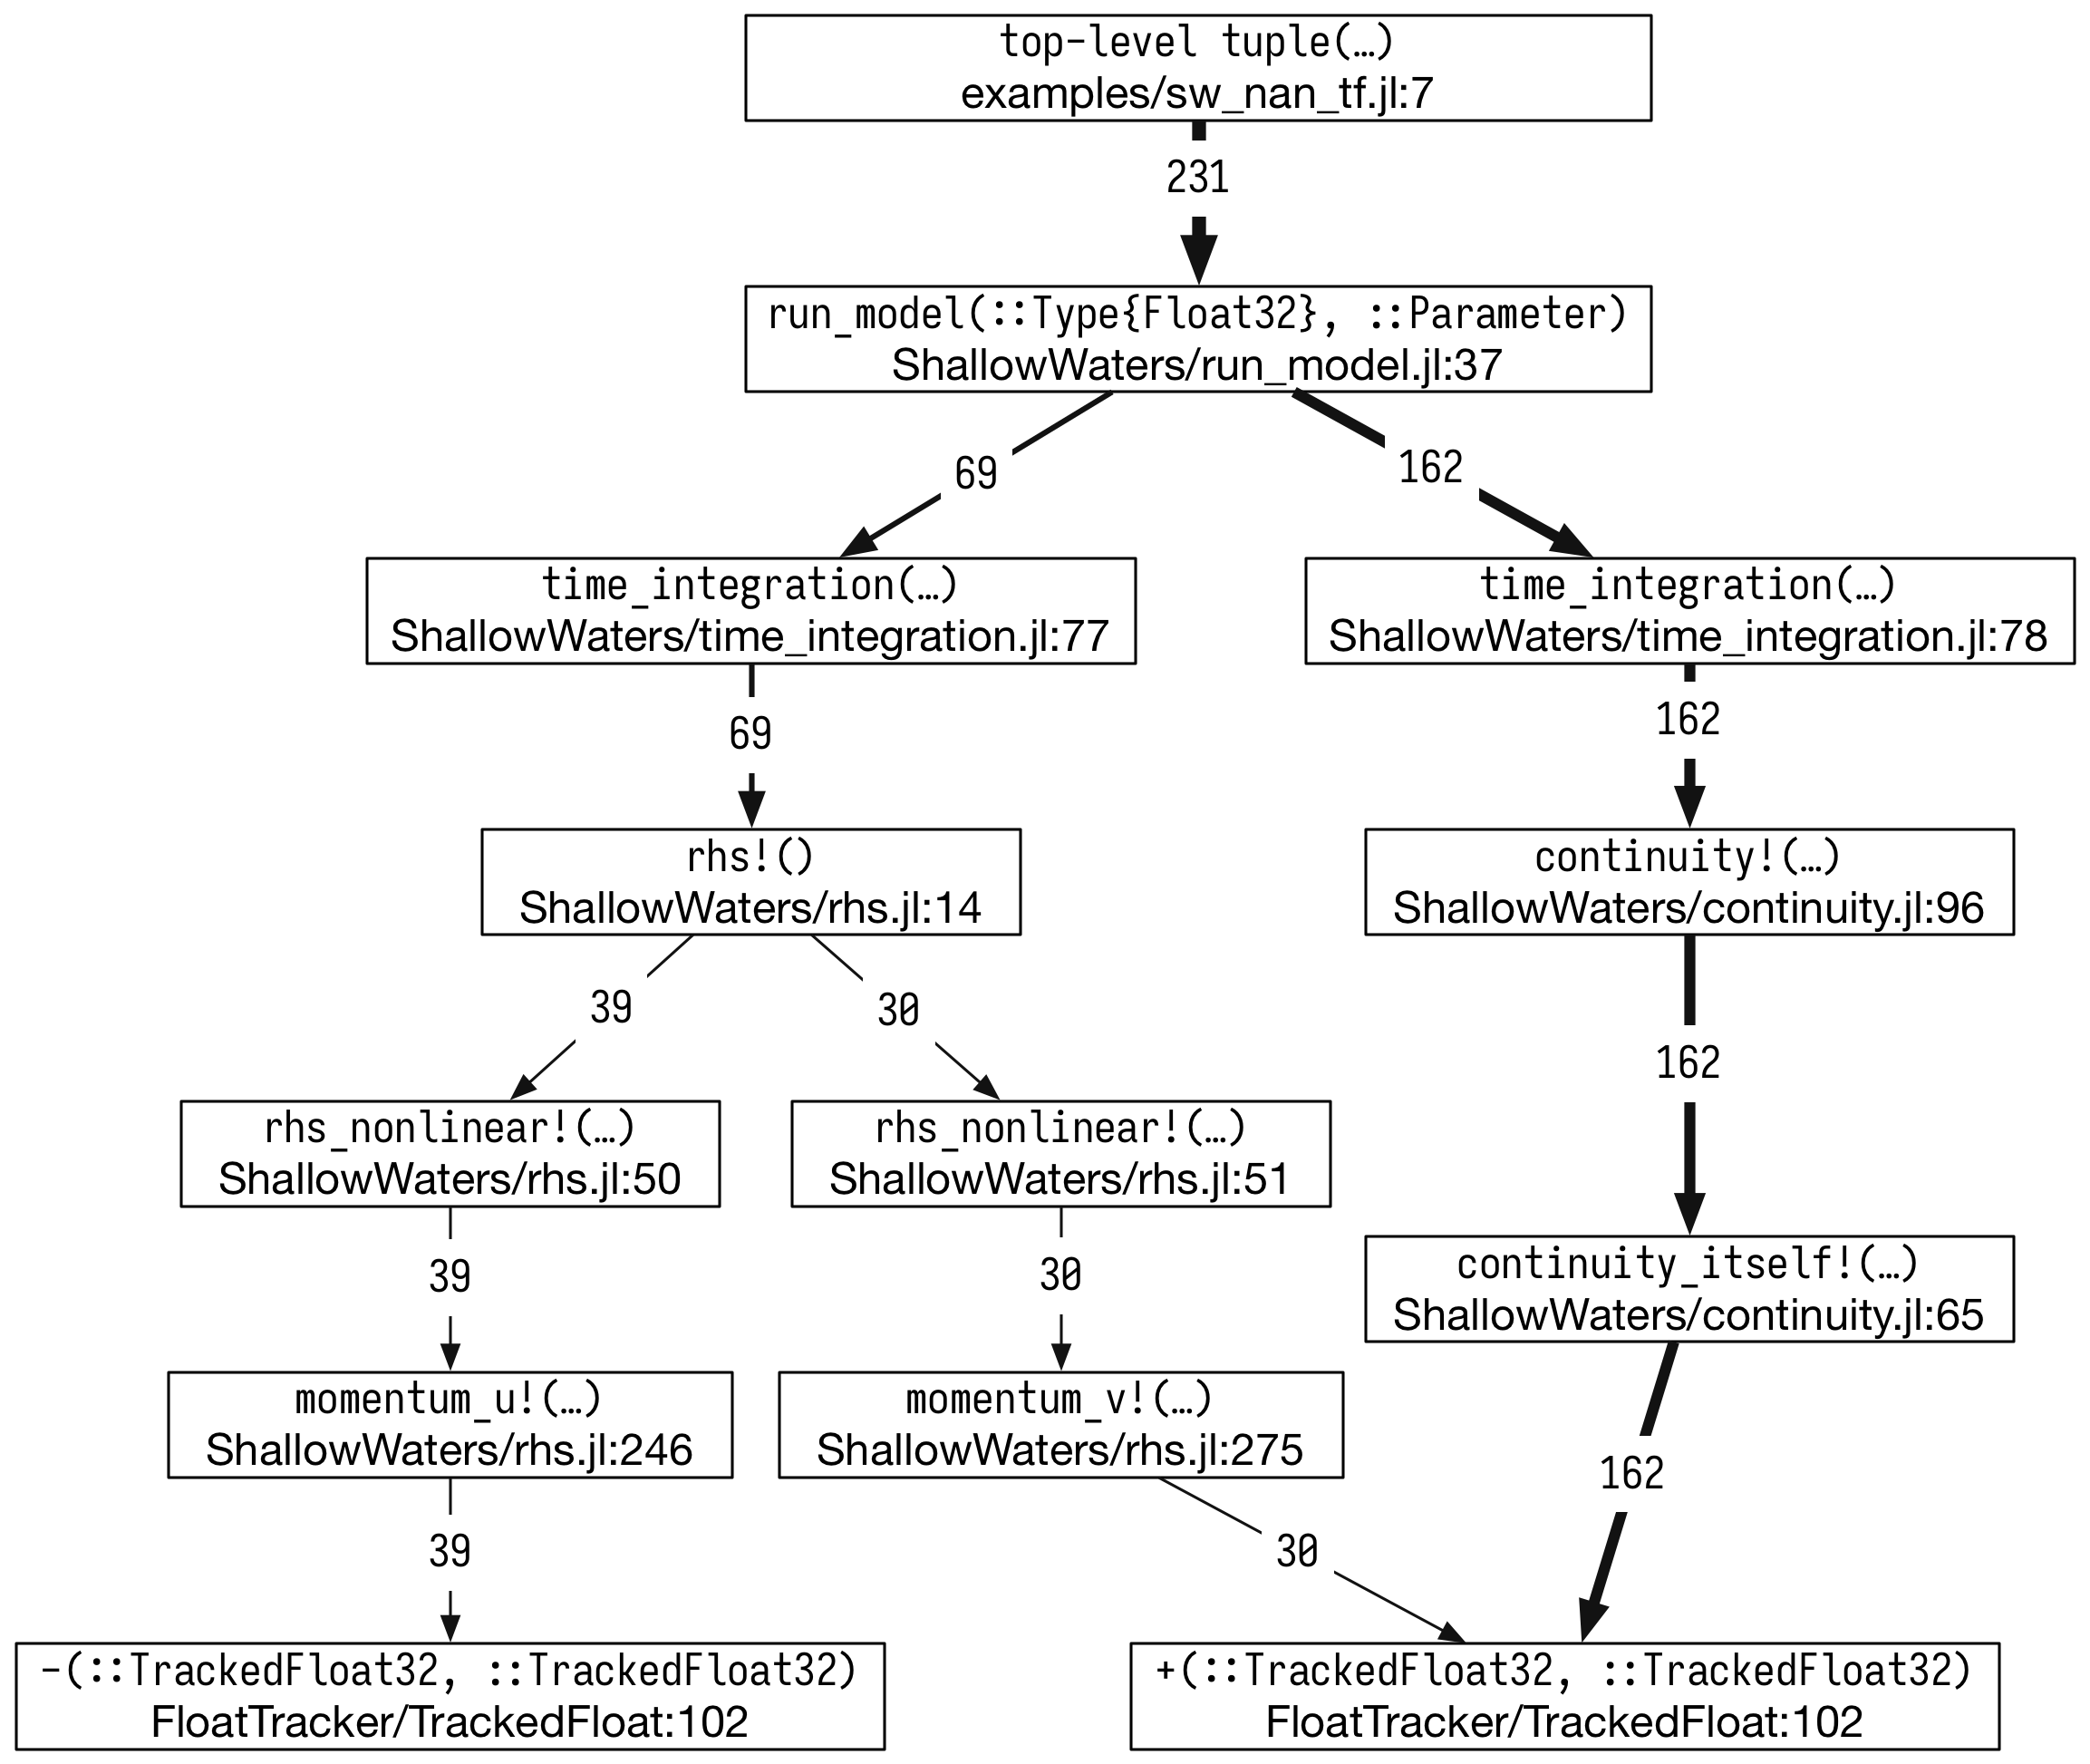
\includegraphics[width=3in]{fig/sw_nan_cstg_clean.png}
  \caption{CSTG of \NaN{} generation logs from ShallowWaters.}
  \label{fig:sw_nan_cstg}
\end{figure}

\begin{figure}
  \centering
  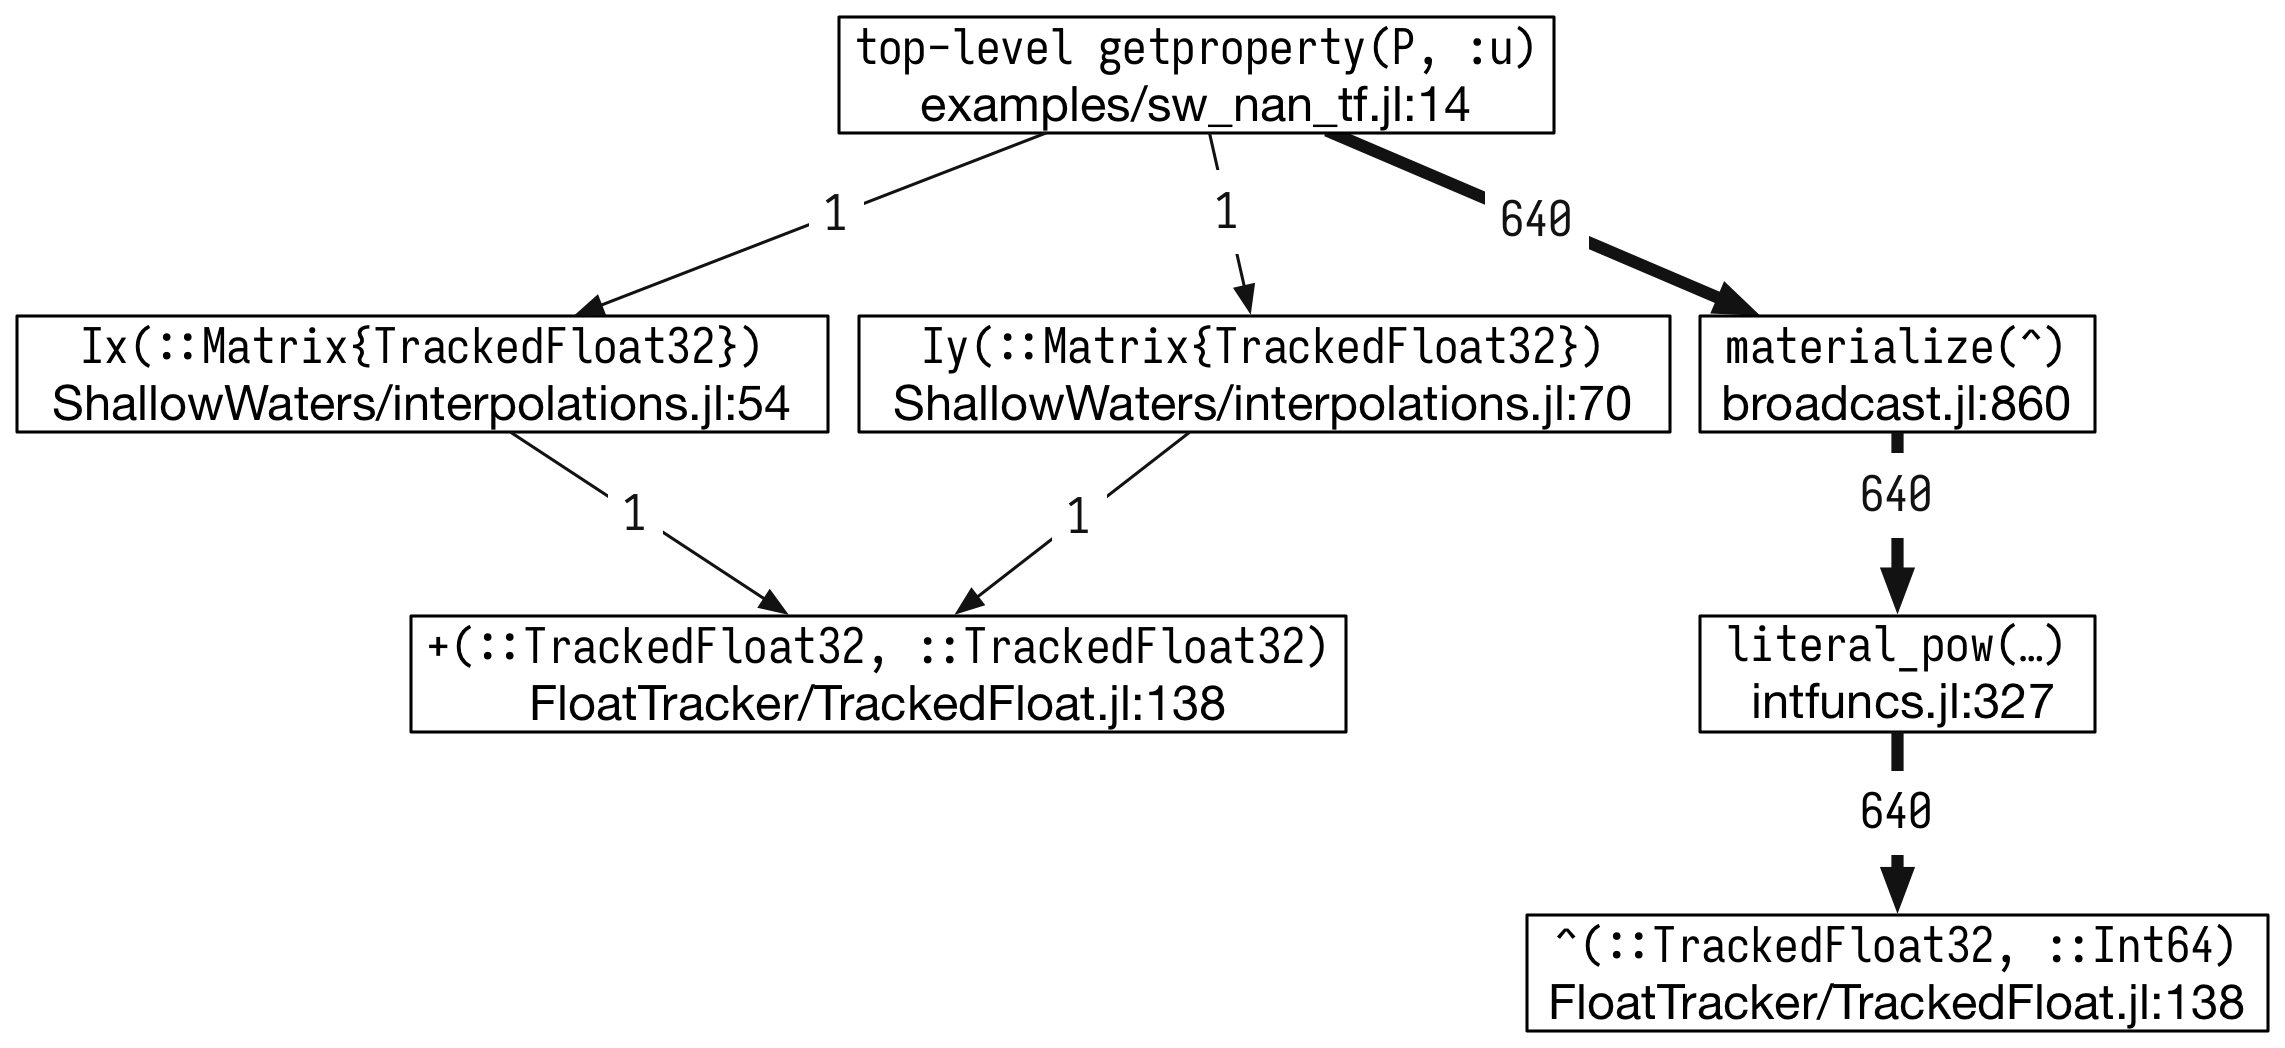
\includegraphics[width=3in]{fig/sw_inf_cstg_clean.png}
  \caption{CSTG of \Inf{} generation logs from the same run as~\cref{fig:sw_nan_cstg}.}
  \label{fig:sw_inf_cstg}
\end{figure}

\subsection{\NaN{} fuzzing to find a kill: OrdinaryDiffEq}

The second thing we evaluated was an N-Body simulation library.
We didn't find any sensible configuration of input parameters that lead to \NaN{} kills like in the ShallowWaters library.
We turned to the \NaN{} injection capabilities of FloatTracker to fuzz the library to find any lurking bugs.
% FIXME: add hyper-ref to § 4.1: ShallowWaters

We configured FloatTracker to inject a single \NaN{} to see if we could find any \NaN{} kills.
On some runs we noticed that we would get a kill and the program would warn about a \NaN{} and prepare to exit.
Contrary to the error message's claim, however, the program went into an infinite loop.

The logs lead us to a routine in the widely-used \texttt{OrdinaryDiffEq} library.
During initialization, a \NaN{} got injected during the execution of \texttt{-} between two \texttt{TrackedFloat}s:

\begin{verbatim}
…
-            at FloatTracker/src/TrackedFloat.jl:89
#__init#628  at OrdinaryDiffEq/src/solve.jl:106
…
\end{verbatim}

That injection point is here on third line of this snippet, which corresponds to line 106 from the \texttt{solve.jl} file in the \texttt{OrdinaryDiffEq} library:

\begin{lstlisting}[language = Julia]
tType = eltype(prob.tspan)
tspan = prob.tspan
tdir = sign(tspan[end] - tspan[1])

t = tspan[1]
\end{lstlisting}

\texttt{sign} correctly propagates \NaN{}s, so \texttt{tdir} now contains a \NaN{}.

We \emph{could} trace this variable through the code, but that would be a lot of grunt work.
Instead, we can look at the \NaN{} kill logs to get a clue as to where we should look next:

\begin{verbatim}
…
<       at FloatTracker/src/TrackedFloat.jl:193
solve!  at OrdinaryDiffEq/src/solve.jl:515
…
\end{verbatim}

We get a very large kill file from this run, and the two lines from above show up repeatedly.
Thus, this is a good candidate location for where the cause of the loop is.

The relevant part of \texttt{solve.jl} looks like this:

% Note for Ashton:
% file here: ~/Research/ode_debug/dev/OrdinaryDiffEq/src/solve.jl
% see line 514

\begin{lstlisting}[language = Julia]
while !isempty(time_stops)
  while tdir * t < first(time_stops)
    # do integration work
  end
  pop_if_work_done(time_stops)
end
\end{lstlisting}

The problem here is on line 2 when \texttt{tdir} is \NaN{}: multiplication propagates \NaN{}s, and comparison kills it, so the condition on the inner \texttt{while} loop is \emph{always} false.
No work got done in the inner loop, and so the conditional \texttt{pop} routine never reduced the size of the \texttt{time\_stops} vector.

Our kill logs led us right to this line; this is a perfect example of how \NaN{} kills can influence control flow to go awry.
In this case, the problem was apparent besides what our logs told us and it manifested as an infinite loop.
More dangerous cases can occur when the influence of a bad comparison is not as readily observable.

\subsection{Finch}
\label{s:finch}

Finch is a domain-specific language for specifying
PDEs~\cite{heislerFinchDomainSpecific2022}.\footnote{Not to be confused
with the Finch loop optimizer~\cite{adka-cgo-2023}.}
In the spirit of FEniCS~\cite{fenics} and related
tools~\cite{freefem,openfoam,dune,firedrake},
Finch helps scientists quickly convert math into code.
What sets Finch apart is its flexibility.
It supports multiple discretization methods (finite element and finite
volume) and multiple backends (Julia, \CPP{}, \Dendro{}~\cite{dendro}).
Furthermore it strives to output code that humans can easily fine-tune.

Fuzzing with \FT{} revealed two places where Finch needed
protection against user input.
The first was when reading an input mesh.\footnote{\urlaccess{https://github.com/paralab/Finch/issues/16}{2023-06-06}}
A \NaN{} injected in the mesh led to a crash further on:
\begin{verbatim}
  BoundsError: attempt to access 1-element
   Vector{Int64} at index [2]
\end{verbatim}
Defensive programming solves the issue.
The second place was in setting bounds for the
solver.\footnote{\urlaccess{https://github.com/paralab/Finch/issues/17}{2023-06-06}}
Here, a \NaN{} could leave bounds uninitialized, leading to a bounds error.
Additionally, \FT{} and \CSTG{}s have been useful for identifying \NaN{}s that
appear in unstable systems.
%% advection2d, high cfl and high T (time) led to NaN during simulation


\subsection{A Bug-Hunting Safari}

% Notes on RxInfer

We searched GitHub for open issues in Julia libraries involving difficult-to-find \NaN{}s.
In our first batch of issues, we found the \code{RxInfer.jl} library with an issue revolving around \NaN{} detection.\footnote{\url{https://github.com/biaslab/RxInfer.jl/issues/116}}
We offered our tool for the package authors to use, and within a day the authors were able to track down the location of a \NaN{} and fix the issue---all with minimal guidance.


\subsection{\GPUFPX{}: Oceananigans}

Oceananigans~\cite{OceananigansJOSS} is simulation package for incompressible
fluid dynamics that can generate code for Nvidia GPUs.
For example, the following program (from the project readme) simulates turbulance:

\begin{lstlisting}[language = Julia]
using Oceananigans
grid = RectilinearGrid(GPU(),
  size=(128, 128), x=(0, 2π), y=(0, 2π),
  topology=(Periodic, Periodic, Flat))
model = NonhydrostaticModel(; grid,
  advection=WENO())
ϵ(x, y, z) = 2rand() - 1
set!(model, u=ϵ, v=ϵ)
simulation = Simulation(model;
  Δt=0.01, stop_time=4)
run!(simulation)
\end{lstlisting}

\GPUFPX{} provides detailed feedback on this program.
The output in~\cref{f:gpufpx} shows that 21 kernels
appear and generate six floating-point exceptions.
There are three \NaN{}s, one \Inf{}, and two division
by zero errors.
The report is a starting point for further investigation
of the reliability of the example.
%% TODO exactly how?


\begin{figure}[t]\centering
  \begin{tabular}[t]{ll}
    \begin{tabular}[t]{lr}
      \zerocode{-{}- FP64 Operations -{}-} \\
      \code{Total NaN:} & \code{2} \\
      \code{Total INF:} & \code{1} \\
      \code{Total subnormal:} & \code{0} \\
      \code{Total div0:} & \code{2} \\
    \end{tabular}
    &
    \begin{tabular}[t]{lr}
      \zerocode{-{}- FP32 Operations -{}-} \\
      \code{Total NaN:} & \code{1} \\
      \code{Total INF:} & \code{0} \\
      \code{Total subnormal:} & \code{0} \\
      \code{Total div0:} & \code{0} \\
    \end{tabular}
  \end{tabular}
  \begin{tabular}{lr}
    \zerocode{-{}- Other Stats -{}-} \\
    \code{Kernels:} & \code{21}
  \end{tabular}

  \caption{Example \GPUFPX{} output}
  \label{f:gpufpx}
\end{figure}


\section{Related Work}
\label{s:related}

Error analysis, typical answer.
Difficult.
CITE

Toronto McCarthy lightweight plotting approach.
No tool support.

Herbie, improving accuracy automatically.
ParetoHerbie

%% http://eprints.maths.manchester.ac.uk/2873/1/fami22.pdf
%% https://drive.google.com/drive/folders/1HkgMpxi6hsqLSZj9tSnuCxnFExPPjmvx?usp=sharing
%% https://docs.google.com/presentation/d/1ueqzb5QY9YHmtY2DfY_hpN9oufSOcXErLWsJOZQxgzo/edit?usp=sharing
%% https://ieeexplore.ieee.org/document/8916392
%% https://link.springer.com/chapter/10.1007/978-3-319-73721-8_24

%% Demmel, somewhere!
%% https://arxiv.org/pdf/2207.09281.pdf

Sherlogs, ShallowWaters
%% https://github.com/milankl/Sherlogs.jl
%% sherlogs

FPSpy x86 binaries [10]
Dinda etal hpdc 2020

FPChecker, " considers CPU OpenMP and MPI codes, again using LLVM
instrumentation"~\cite{ltlg-iiswc-2022}

6-8,24,25
Arnab Das scalable yet rigorous
Marc Daumas Certification of Bounds Expres
David Delmas Towards an Industrial Use of
Alexey Solovyev FPTaylor Results table
Titolo absint


CSTG~\cite{hmbdrg-cse-2014}.
What else???

GPU-FPX state of art, companion project~\cite{llsflg-hpdc-2023}.
Latest in line of work.
BinFPE exn checking, slower than GPU-FPX, 
\cite{llg-soap-2022}.
FPChecker, early pioneer, fpx in gpus, llvm-level instrumentation
if compiled with Clang, but most gpus use closed NVCC compiler~\cite{l-ase-2019}.



\section{Discussion}
\label{s:discussion}
% future work

\subsection{Performance}
\ref{s:discussion-performance}

% TODO: citations!!!!
% TODO: real numbers!!!
\FT{} incurs significant overhead on the order of 100x slower than a non-instrumented run of the same program.
To put this number into context, Valgrind runs with a similar level of slowdown.

In addition to the cost incurred by intercepting \fp{} operations, gathering stack traces is expensive---we measured a significant slowdown on the order of 10x relative to a non-logging setup of \FT{}.
We recommend that users of \FT{} make use of the \texttt{maxLogs} and \texttt{exclude_stacktrace} configuration options to limit the number and kind of logs gathered, and thereby reduce the number of calls to \texttt{stacktrace()}.

\subsection{Tracking more than \NaN{}s and \Inf{}s}
FloatTracker is capable of monitoring all sorts of events in a \fp{} value's lifetime---not just a value going to \NaN{} or \Inf{}.
We spent most of the time engineering and testing \NaN{} tracking and injection.
Adding \Inf{} tracking took a few hours.
Adding other values of interest presents no fundamental difficulties.

\subsection{Enhanced Fuzzing}

While fuzzing is useful for discovering issues, its success rate
is low because \emph{every} \fp{} operation is a candidate
for injection.
Even operations that are already well-defended against \NaN{}s are candidates.
\FT{} could use two sorts of tools for improving injection.
First, fine-grained control to let users decide where not to inject.
Second, tools for understanding the context of an injection point
after the fact.
Program slicing is especially relevant to the latter point (and effectively
what we did by hand when fuzzing Finch~\cref{s:finch}).
For each operation, an expert needs to study the values that feed into it to
decide whether they are protected or not.

%% TODO example, start here at glbvertex https://github.com/paralab/Finch/blob/master/src/grid.jl#L360

\subsection{Static FPX, Gradual Types}

FILL


\section{Acknowledgments}

We would also like to thank the developers of \code{RxInfer.jl} for feedback on \FlowFPX{}.

% **************GENERATED FILE, DO NOT EDIT**************

\bibliographystyle{juliacon}
\bibliography{ref.bib}


\end{document}

% Below is some Emacs-specific stuff. If you're using Emacs, you should try
% using the new jinx package for spell-checking!

% Local Variables:
% jinx-local-words: "CFL CSTG's CSTGs Courant Friedrichs JuliaHub Lewy OrdinaryDiffEq RxInfer ShallowWaters Sherlogs TrackedFloat isnan"
% citar-bibliography: ("./ref.bib")
% End:
